\documentclass[]{tufte-book}

% ams
\usepackage{amssymb,amsmath}

\usepackage{ifxetex,ifluatex}
\usepackage{fixltx2e} % provides \textsubscript
\ifnum 0\ifxetex 1\fi\ifluatex 1\fi=0 % if pdftex
  \usepackage[T1]{fontenc}
  \usepackage[utf8]{inputenc}
\else % if luatex or xelatex
  \makeatletter
  \@ifpackageloaded{fontspec}{}{\usepackage{fontspec}}
  \makeatother
  \defaultfontfeatures{Ligatures=TeX,Scale=MatchLowercase}
  \makeatletter
  \@ifpackageloaded{soul}{
     \renewcommand\allcapsspacing[1]{{\addfontfeature{LetterSpace=15}#1}}
     \renewcommand\smallcapsspacing[1]{{\addfontfeature{LetterSpace=10}#1}}
   }{}
  \makeatother
\fi

% graphix
\usepackage{graphicx}
\setkeys{Gin}{width=\linewidth,totalheight=\textheight,keepaspectratio}

% booktabs
\usepackage{booktabs}

% url
\usepackage{url}

% hyperref
\usepackage{hyperref}

% units.
\usepackage{units}


\setcounter{secnumdepth}{2}

% citations
\usepackage{natbib}
\bibliographystyle{apalike}

% pandoc syntax highlighting

% longtable
\usepackage{longtable,booktabs}

% multiplecol
\usepackage{multicol}

% strikeout
\usepackage[normalem]{ulem}

% morefloats
\usepackage{morefloats}


% tightlist macro required by pandoc >= 1.14
\providecommand{\tightlist}{%
  \setlength{\itemsep}{0pt}\setlength{\parskip}{0pt}}

% title / author / date
\title{环境黑板报}
\author{805}
\date{2017-11-23}

\usepackage{booktabs}
\usepackage{ctex}
\setCJKmainfont{FangSong}
\setCJKmonofont{KaiTi}
\setCJKsansfont{SimHei}

\begin{document}

\maketitle



{
\setcounter{tocdepth}{1}
\tableofcontents
}

\chapter{念念不忘 必有回响}\label{-}

\textbf{广播站王站长}

行走在市区的环路上,穿插于市郊的街巷间,随处可见十九大的最新标语:``不忘初心,牢记使命''。环路上,有车水马龙的喧嚣;街巷间,有贩夫走卒的吆喊。初秋的北京,雄心壮志也很难抵挡供暖前的寒冷。在这座底蕴深厚、庄重方正复又灯红酒绿的都市里,每天面对拥挤的人潮和日复一日的生活,我常常会扪心自问:``究竟何为初心?''

初心常常不语。

要说来,环境专业其实是一个偏于冷门的小专业,在我刚上大学那会,环境学院一届就两个班,五十几号人;上研究生的时候一届也不到一百个学生。这么小的学院,如果非要说有什么优势,那就是女生比男生多,而且质量还不错。读博期间,那些二十七八岁,脱去白大褂立刻成为泪朱砂的妙龄女博士们,着实是枯燥科研生活中的一道风景。

随着北京雾霾的爆发,环境问题开始越来越被人们所熟知,然而环境这一行当却并没有跟着一起爆发式成长起来,因此对于环境人来说,就业常常是一个痛苦的选择。我大学里特别好的一哥们,也是我的室友,他留学日本,在土壤修复上苦读五年,博士学成归来,毅然决然地前往了------碧桂园。当他拿着大约是我三倍的工资,在世界各地自由飞翔的时候,我依然在这半径半里的地方,重复着读博时的生活,这大概就是所谓一花一世界,一叶一菩提。

如今大学时一个学院的同学少有还在环境这个相关的行当里,因为这个行当既苦且窄。若从进入这个专业算起,已经过了大约十二年的时光。十二年,足以让你当年暗恋的女孩嫁为他妇;足以将年轻的校草喂成油腻大叔,但同样的十二年,如果我们还坚持在这个最开始的选择上,能不能算作是初心不改?如果可以,这大概能作为我们办这个公众号的一个初衷吧。

初心不改,就应该完成一些使命。是的,北京雾霾的时候,你知道了雾霾的可怕,那南方空气中的氮、硫化合物就不可怕么?室内空气中的甲醛和VOC就不可怕么?土壤中迁移的砷和汞就不可怕么?你知道每年有多少的农药、重金属和持久性有机污染物进入到环境么?你知道每天在聒噪的声环境状态下生活对身心会造成多大的创伤么?\ldots{}\ldots{}是的,真相常常触目惊心,我们不能等到雾霾来袭的时候才知道治理大气,更不能等到水源枯竭的时候,才知道珍惜水源。如果作为环境人我们也回避这些责任,那人与自然和谐相处的中国梦恐怕也只是空谈。

正因为如此,作为一群正在三十岁当口的环境人,我们有气力、有精力更有愿望撸起袖子干起来。在我们的队伍中,有在海外读博后,随意一篇随笔就能被科学网主页转载的科院小飞侠;有在高校里谈笑间文章与项目齐飞的青年才俊;既有从环保机关到地方监测站的一线骨干;更有大国企到民营企业环境项目的一手负责人;最不济的大概就是我这样留在科学院里,守着自己一亩三分地的人了。我们愿意用一个平台去展示一下我们的工作,不需要一定摆出科学的姿态佩戴高大上的光环,我们更愿意去讲述一些故事,如果把我们的心路历程呈现出来,其实是一部环境人的血与沙。

因此我们更想去展示一些实实在在的东西,更希望推送的每一篇文章都言之有物。环境访谈、热点解读和前沿动向将是这个公众号最主要的推送方向。这些东西,或在天边、或在眼前、或有所耳闻、或已然亲历。这些内容,科研的、政策性的、工程项目的、经历感悟的,简而言之,我们希望来访的每一个人都能在公众号的不同模块中找到一些共鸣、读出一些趣味,都能感受到作者撰写每一个字的用心。如果一不小心,刚好帮助到解决你的困惑或者其他实际的问题,那对我们而言,真的是初心有值了。

在这之外,我们是一群很有趣也很有范的人,同时也为了增加公众号的受众,我们也愿意分享一下环境人的生活日常。我们的生活也许不尽如人意,但我们的文字一定充满情趣,疲劳之余来此闲读,倒也是消磨时间的好去处。同时更希望这个公众号能成为一个交流的平台,我们可以在这里谈天说地、交友论道而共同进步\ldots{}\ldots{}但我们拒绝黄、拒绝赌、拒绝黄赌毒。

鲁迅先生说:``愿中国青年都摆脱冷气,只是向上走,不必听自暴自弃者流的话。能做事的做事,能发声的发声。有一分热,发一分光。就令萤火一般,也可以在黑暗里发一点光。不必等候炬火,此后如竟没有炬火,我便是唯一的光。''我们不奢求去做唯一的光,但我们愿意和大家一起发光来照亮前路。

开篇数语,不过投瓦砾以引玉珠,愿这个公众号能越办越好,也希望再过十二年,眼前的这些人能够依旧初心不改。

黑板报计划一周一更,多谢关注,我们下周见\ldots{}\ldots{}

\chapter{雾霾专题}

\section{混沌的冬日}

\subsection{序}

1962年,美国海洋生物学家 Rachel Carson
出版了《寂静的春天》,这本书展示了农药污染下没有虫鸣的春天。在其影响下公众开始关注环境污染问题并开启了环境科学研究的序幕。然而,国内公众对于环境污染的关注也许并不用等到春天。近几年,每每国庆刚过,雾霾就会几次三番的席卷全国,呈现出混沌的冬日。

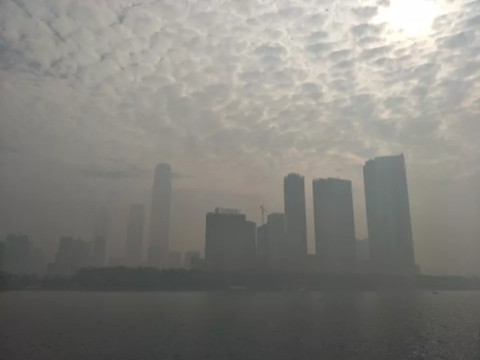
\includegraphics[width=18.61in]{images/cw1}

有人说发展的问题会在发展中解决,例如发达国家也经历过类似的阶段,但伴随产业转型与法规调控,污染问题都会自然而然地消亡;又有人说虽然城市会被雾霾笼罩,但从统计数据上看居民平均寿命其实比所谓田园风光的乡村更长;还有人说大气污染相比土壤、水还有固废污染都不算严重,只是可见度更高(也就是能见度低)\ldots{}\ldots{}的确,雾霾这个现象背后有着错综复杂的社会经济影响,从不同的角度去看会发现不一样的东西。多一个角度看问题并不会让你过的更好,但至少更明白些。

下面我将给出一些非技术与法规调控的视角,希望对读者理解雾霾以及其他一些环境污染问题能有帮助。

\subsection{研究增长的极限}

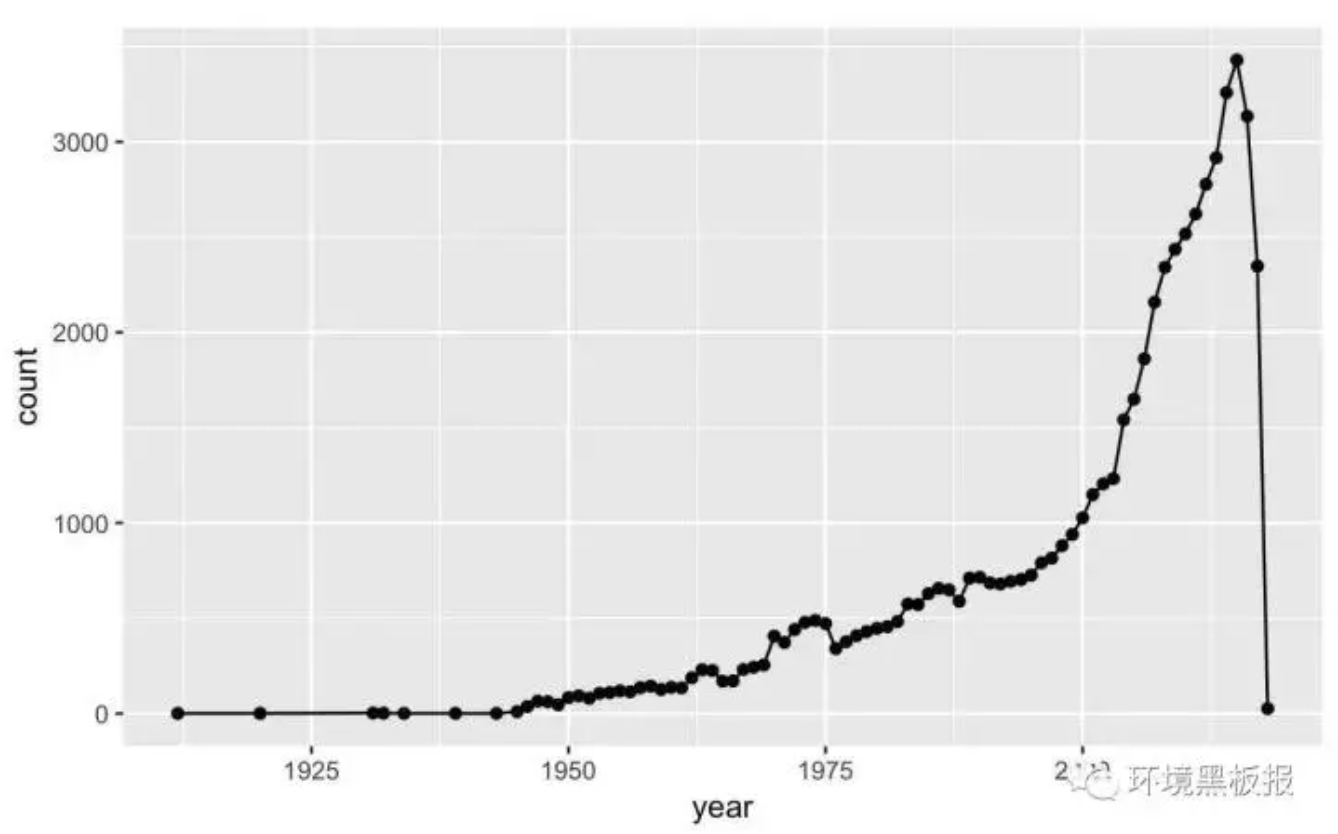
\includegraphics[width=18.58in]{images/cw2}

上图是生物资讯数据库 Pubmed 上用颗粒物(particulate
matter)作为关键词得到的论文数量,一百年来可以说是持续增长,特别是21世纪以来增长尤为迅猛。但需要注意的是到2015年达到了峰值(3429),16年已经明显下降(3134),今年还有两个月(2348),但不出意外也不会超过16年。至于为什么会有少量18年文献(26),这是学术界硬通货论文的通货膨胀,透支未来可以说是现代社会最伟大也最危险的发明,学术界亦然。也就是说,对于颗粒物的研究兴趣实际已经在降低了。

这个现象可能有点反直觉,因为近几年大气环境污染的公众关注度非常高,经费投放也很可观,但学术界却降低了学术交流频次。无独有偶,使用传统研究热点例如汞、铬、二恶英、基因组、纳米颗粒去进行检索,都会发现研究在2014-2015年间出现了峰值。但同时如果去看一些新兴研究例如3D打印,颗粒物中的细颗粒物(fine
particulate
matter),则增长还是非常迅速的(下图是以细颗粒物为关键词的文献发表状况)。

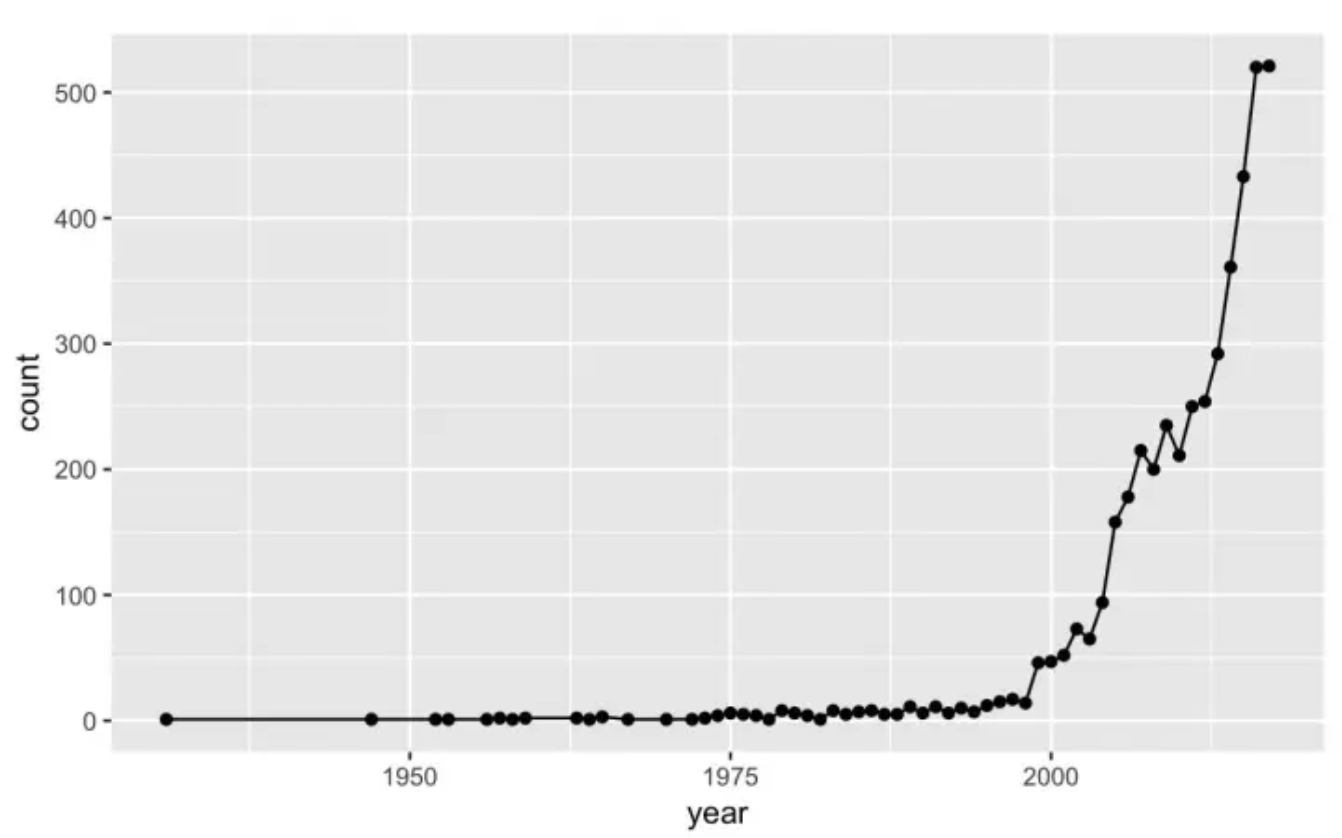
\includegraphics[width=18.64in]{images/cw3}

如果把学术界所有人的研究精力看成是总量稳定的,那么论文数可以看成精力的指标,对于包括大气颗粒物在内的很多环境研究课题而言,学术界正在把蛋糕切给更新的技术与概念。同样是进行雾霾研究,如果你从事微米尺度研究,而学术界却更加认可纳米尺度的研究,那么你的文章就很难发表,然后就是经费紧张,如此循环;进而使得新概念也不断变成老概念。

就颗粒物研究而言,目前学术圈总体关注度已经在下降,但分支中却有上升的。那么可想而知,学科内存在激烈竞争,并不是所有的颗粒物研究方向都是热点。而且还可以预期的是少数研究方向的异军突起会吸收更多学科内的研究资源,很多优秀的研究人员可能一开始选错了研究方向,最终的结局就是转行。研究的增长极限是客观存在的,所以如果你在这个年代打算去找专家咨询,最好去问上升期的新人,因为很多概念从出现到流行不到三五年,有经验的专家反而可能因为有学科内竞争关系而给出带有其自己都意识不到的感情色彩的论断。

\subsection{有原罪的雾霾}

如果某天PM2.5爆表,然后你又恰好感觉到嗓子不舒服,那么很自然你会认为这是雾霾的锅。这符合情理,但不一定符合事实,雾霾跟健康是有联系的,但跟健康有联系的可不仅仅是雾霾。即使仅仅考虑大气污染,颗粒物也只是能够产生爆表AQI的一个因素,其余的例如工业主导的硫酸型烟雾或汽车尾气主导的光化学烟雾都会影响健康,都能让嗓子不舒服,此时你会把原因归到哪里?

进一步讲,环境因素也只是影响健康的一个方面,遗传也起作用。假如你在雾霾天听到一个有气管炎家族病史的患者在咳嗽,你会认为是环境影响还是遗传作用?而根据最近Science的一份研究,即便你排除掉环境因素与遗传因素,仅仅是新陈代谢过程中DNA的复制次数就可解释癌症的发病率的66\%,而这个过程根本就无法用先天后天因素来解释,就是个生长问题。

在中国,雾霾是有原罪的,它实际承载了社会转型期人们的一部分焦虑。如果其对健康的总影响是十,那么其中真实作用可能也就二三,替遗传和其他污染物背了三四的锅,还有三四则可以说是心因性的。今年柳叶刀上一篇文献就提到,中国PM1跟PM2.5大概贡献了医院急诊的4.47\%与5.05\%。这种研究有两个问题,第一,即使排除了意外导致的急诊(例如车祸),就诊行为本身就会受天气影响;此外就是
type M
型错误(效应数量级错误),也就是说这个效应是真实的,但是影响不一定大。

这其实是目前环境研究的一个通病,找一组病人和一组正常人(有的连这个也省了)采集样本,然后一把测定几百上千种污染物(这个现在技术上是没问题的),然后算相关系数,这种情况随机你都可以发现几个的,而这样做出的发现有个通病,那就是效应通常不大,很难重现。一个小而真实的效应或许有学术价值,但舆论一放大就会产生公众心理焦虑,而心理状态又会影响生理状态,这类影响可能并不比真实影响小。

雾霾是有原罪的,但被过度聚焦了,由此产生的焦虑与恐慌本身也会产生健康影响。如果公众可以更好理解科学研究现状与其中的问题,这并不能客观降低空气污染的健康影响,但在实际意义上却可能减轻雾霾的心因性副作用。

\subsection{万金油的幻象}

不知道从什么时候开始,万金油的心态重新出现了。以前如果我告诉你有一种方法可以让你永远远离雾霾危险,你肯定说我瞎扯。好,现在我换一种说法,在人工智能+区块链+可穿戴设备+大数据的实时监控下,我可以给你一副智能眼镜,上面会实时反应你现在的风险指数,如果指数超过80\%,那么你就应该进入室内。逻辑上来说,如果你按照超过指标就躲到室内,那么这个风险永远不会变成100\%,也就是说,这跟我刚才说的永远远离雾霾危险实质等同,但是这样的产品你多半不会觉得是瞎扯,甚至会愿意付高价购买,这又是为什么?

万金油思维从来都没远离过我们,只是从熟悉的名词变成了看似专业的术语。人们有一种看起来很理性但又很荒谬的行为:乐观而盲目地相信着未知的科技。雾霾来了,那就买个最好的空气净化器;外面看不见了,那就来个3M口罩;嗓子不舒服了,那就去搞点清肺的保健品。其实很多人都知道这些科技可能还不成熟,但只要花钱了就有种事情完结可以甩锅的想法。真实的情况往往是越是大家关注的事物,就越有人去贩卖这种包装过的万金油,你买到的更多只是一个确定性的心态。

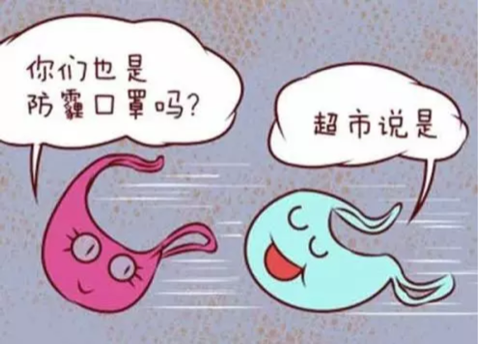
\includegraphics[width=13.81in]{images/cw4}

在这个分工细致的现代社会里,绝大多数的服务业出售的都是经过专业化包装的确定性,用来抵消分工后一颗颗螺丝钉无法感知全局的焦虑。雾霾就是个全局问题,涉及很多不同专业的知识,当个体被复杂性搞晕时,最简单的方法就是掏出一把钞票买个心安理得。即使问题不能在当前根本解决,但生活总要继续,或许这就是万金油思维在进化上的意义。在雾霾这种大IP下,科学家、政府、骗子、掮客、投机商你方唱罢我登场,过分认真你就输了。

\subsection{混沌的冬日}\label{-1}

回溯千年,宋代诗人陆游在《秋霁》中提到:``驱除云雾极知难'',除了难在技术与法规,雾霾也是直指人心的。

看看窗外,凛冬将至

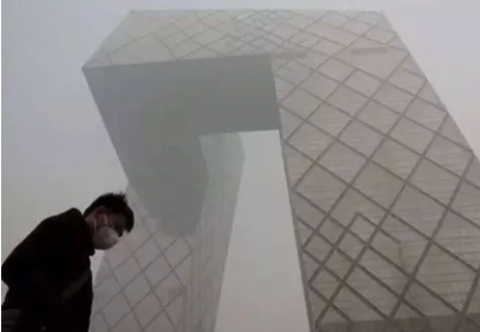
\includegraphics[width=14.94in]{images/cw5}

作者:yufree 编辑:栟

\chapter{城市生态}

\section{城市之殇}

\subsection{序言}

2012年7月21日,一场61年一遇的大暴雨让北京成为``汪洋水城'',想不到有生之年居然可以在帝都这个缺水的城市同时实现了``山盟海誓''。无独有偶,不仅北京遭遇了这样的窘境与困惑,其他城市诸如南京、武汉、广州、杭州等也先后开启了``看海模式'',这种``城市之殇''已经成为近年来城市发展挥之不去的阴影。

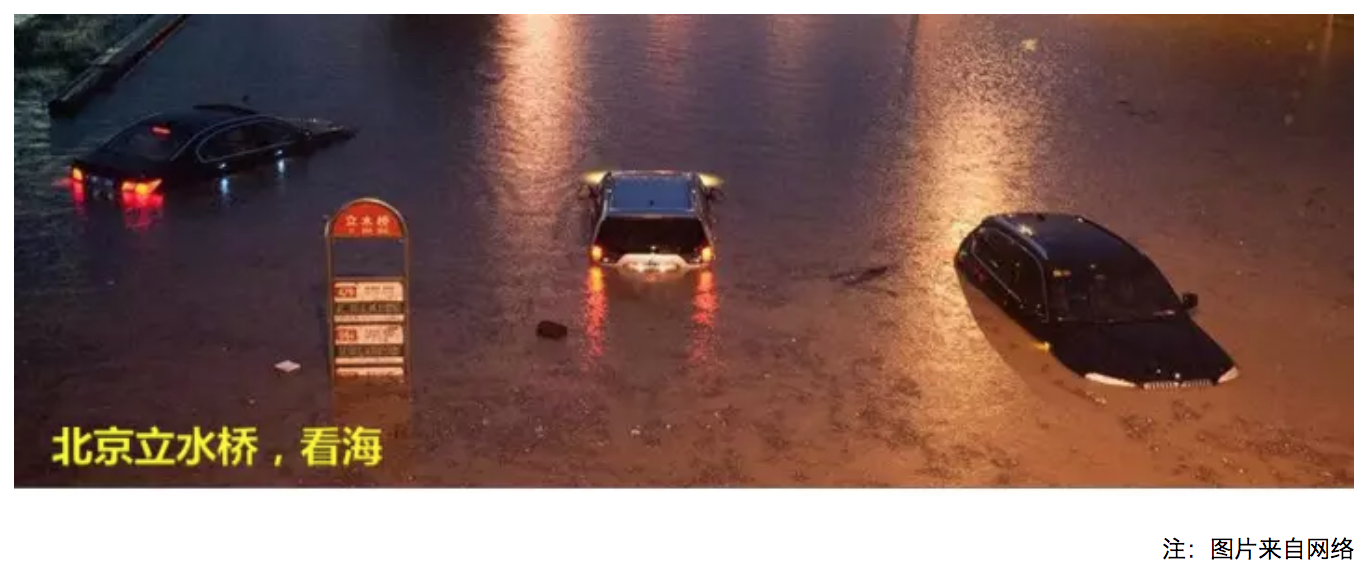
\includegraphics[width=19in]{images/ch1}

那么,为什么我们城市的排水能力一遇到暴雨甚至中小雨就原形毕露?这就有必要来聊一聊本期的话题:``海绵体''。海绵体,顾名思义,是一种对蓄水的形容,自然界原本是一个巨大的海绵体,而如今城市的爆发式发展建设已严重破坏了自然的海绵体,损害了自然的水循环系统。传统的城市建设模式根本不具备应对超标雨水的能力,那么必然会导致``逢雨必涝'',同时还会带来水环境污染、水资源紧缺、水安全缺乏保障等问题。

2013年12月12日,习近平总书记在《中央城镇化工作会议》的讲话中强调:``提升城市排水系统时要优先考虑把有限的雨水留下来,优先考虑更多利用自然力量排水,建设自然存积、自然渗透、自然净化的海绵城市''。海绵城市顺应时代号召应``运''而生。

\subsection{海绵城市是什么}

海绵城市的理念其实在我国古代早已践行,比如故宫的排水系统、云南的``哈尼梯田''模式、赣州的``福寿沟''蓄排系统等,都算作是早前的雏形。若要刨根求底地问海绵城市是什么,海绵城市更多的是一种新型的城市发展模式。

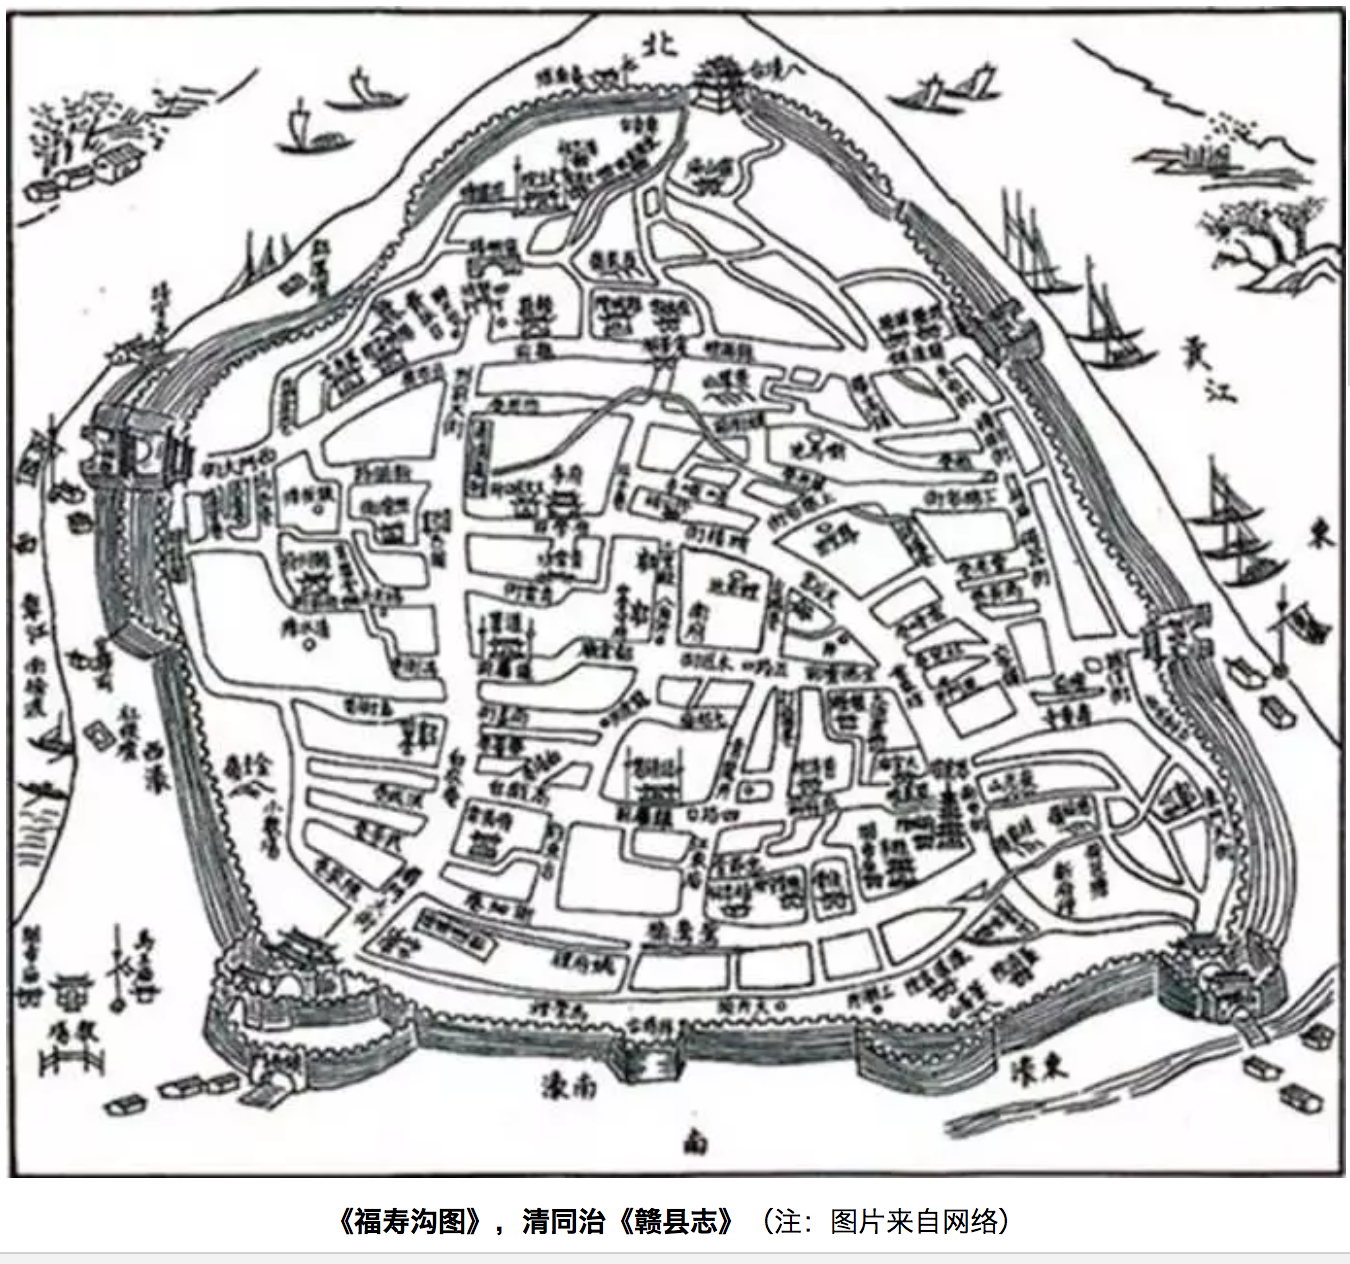
\includegraphics[width=18.75in]{images/ch2}

海绵城市的初衷是让城市能够像海绵一样,在适应环境变化和应对自然灾害等方面具有良好的``弹性''。简单来说,下雨的时候,城市可以像海绵一样吸水、蓄水、渗水,防止洪涝的出现;在雨水过后,干旱的时候,又可以将蓄存的水``释放''并加以利用。但同时,我们又希望这个``海绵''能发挥更大的作用,比如说还可以净化水体,让雨水在城市存积、渗透的同时得到净化,以利于进一步的雨水资源利用和生态环境保护。这就为海绵城市的设计、建设提出了更高的要求,不单是依靠恢复或构建自然途径来蓄水、存水,还应当结合人工措施来辅以完成水资源的净化、利用和排放。

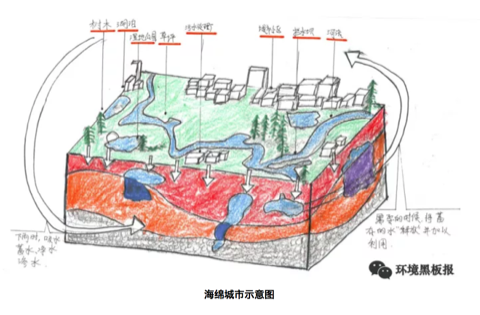
\includegraphics[width=18.56in]{images/ch3}

因此海绵城市的具体建设既不能``窄'',也不能``宽''。太窄就会回到植树造林搞绿化的老路子上去;太宽就会变成``海绵城市一个框,啥都可以往里装''。其实海绵城市建设还是要以目标与问题为导向,运用``源头、中途、末端''的措施,使绿色设施与灰色措施相结合,才能实现真正的目标。

简明地讲,源头主要以低影响开发设施(LID)为主,包括植草沟、雨水花园、生物滞留设施等,中途主要包括:雨水廊道、管网、沟渠等,末端主要包括:湿地、调蓄塘、调蓄池、水系等。

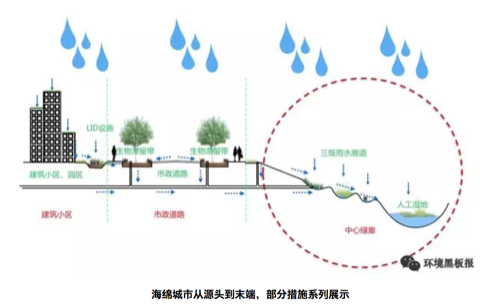
\includegraphics[width=17.89in]{images/ch4}

\subsection{海绵城市试点}

海绵城市的建设借助国家重视生态环境的东风,目前共执行了2个批次、30个城市的试点,试点期3年。期内国家将给予直辖市每年6亿专项补助,省会城市每年5亿,其他城市每年4亿元。

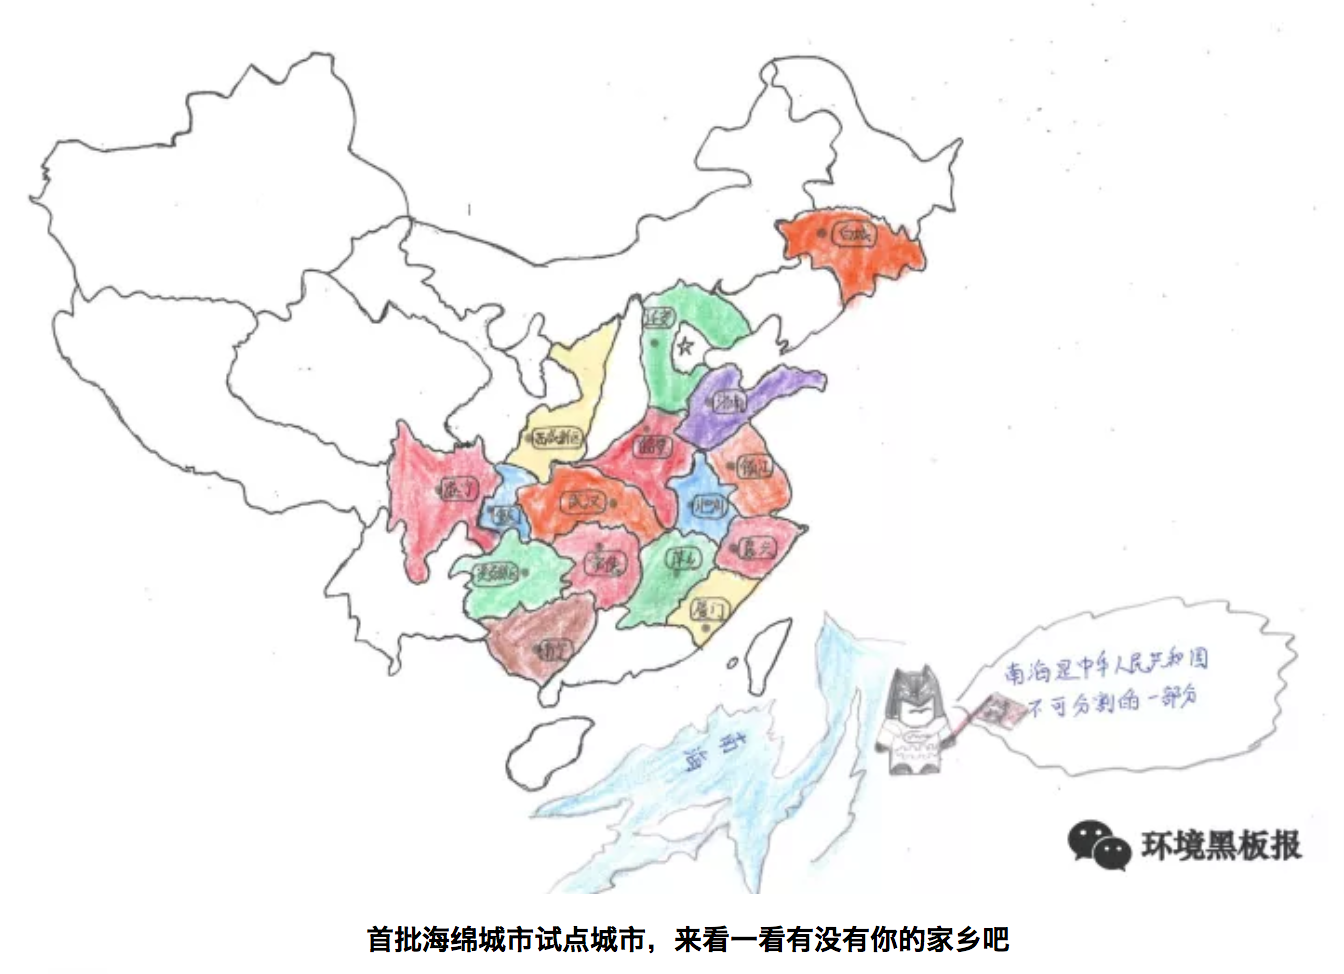
\includegraphics[width=18.67in]{images/ch5}

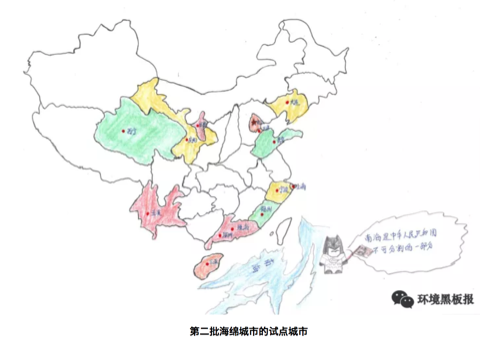
\includegraphics[width=18.92in]{images/ch6}

目前来看,海绵城市建设还没有一个全国性的``统一标准'',主要是因为我国地域差异大,东西南北中,面临的问题与挑战各不相同。比如北方地区多为缺水的寒带地区,南方地区则更容易发生内涝,西部地区多属于湿陷性黄土地区,也极度缺水。因此不同区域的海绵城市建设也应因地制宜。

\subsection{浅谈海绵感悟}

笔者从2015年开始从事海绵城市建设方面的工作,先后参与了多地的海绵城市试点建设的咨询、设计等工作,主要涉及海绵城市建设系统方案编制等方面。这里跟大家分享一下三年多来笔者对海绵城市建设的一些想法与感悟,希望能对现在或将来参与到海绵城市建设中的同仁们有所帮助。

\subsubsection{从管理部门的角度}

如果您是一位相关部门的负责人,笔者虽人微言轻,但也愿意提供一些思考供您参考。
海绵城市的建设是一个很复杂、庞大、时间跨度也大的系统工程。而且里面涉及到很多学科和部门,简单数数就需要规划、市政、园林、水利、道路等专业;住建、水利、园林、环保等部门来互相配合。因此如何统筹规划,通力协作,避免形成各自为政、``九龙治水''的局面,是一门很深的学问。

同时,很多城市现在都有新、老城区,新城区建设制约少、阻力小,一旦方案设计得当,大可一马平川。但是老城区就不一样了,不仅居民多、遗留矛盾和问题多多,牵一发而动全身,搞不好容易激化矛盾。这个时候,就不能只顾海绵城市建设的目标,还要考虑经济承受能力、轻重缓急、资金利用效率、建设时序、社会影响等方面。
千万、千万不能不分轻重地全面开工建设和盲目翻挖。最好可以以解决城市内涝、雨水利用、黑臭治理为突破口,结合棚户区和城乡危房改造、老旧小区有机更新等工作同步推进。

\subsubsection{从项目公司负责人的角度}

当前海绵城市的建设基本上都以项目打包的形式交由PPP公司全权负责建设。如果您是一位项目公司的负责人,首先恭喜您拿下了海绵城市的项目,但是接着愁人的事情来了。在很多项目管理过程中,一些PPP公司``当家不做主'',没有自主权,项目的管控不是由PPP公司独立操作,而会受到相关部门的干预,导致指挥不合理的局面。因此,如果您能在项目开展前和相关部门做好充分的沟通,对您后续工作的开展会有很大帮助。
同时,虽然目前海绵城市都处在建设之中,但是即使这样,试点期也已经过了2-3年,后期的运营维护也该做一些考虑了。如果您公司还没有做这方面的准备,那可千万要小心了,现在环境追责可是很严重的哦。

\subsubsection{从设计师的角度}

如果您是一名规划师或者设计师,请一定要``迈开腿,管好嘴''。一定要多去现场,没有调查就没有发言权,不能板凳一坐就站不起身,嘴皮一碰就出方案。曾经有一位设计院的设计师理直气壮地反驳说没必要去现场看这么细,走了个过场回来,后来设计的时候全部依靠业主来提供信息作为依据。结果可想而知,做出来的设计方案根本经不起推敲,漏洞百出,更别说拿去指导施工建设。

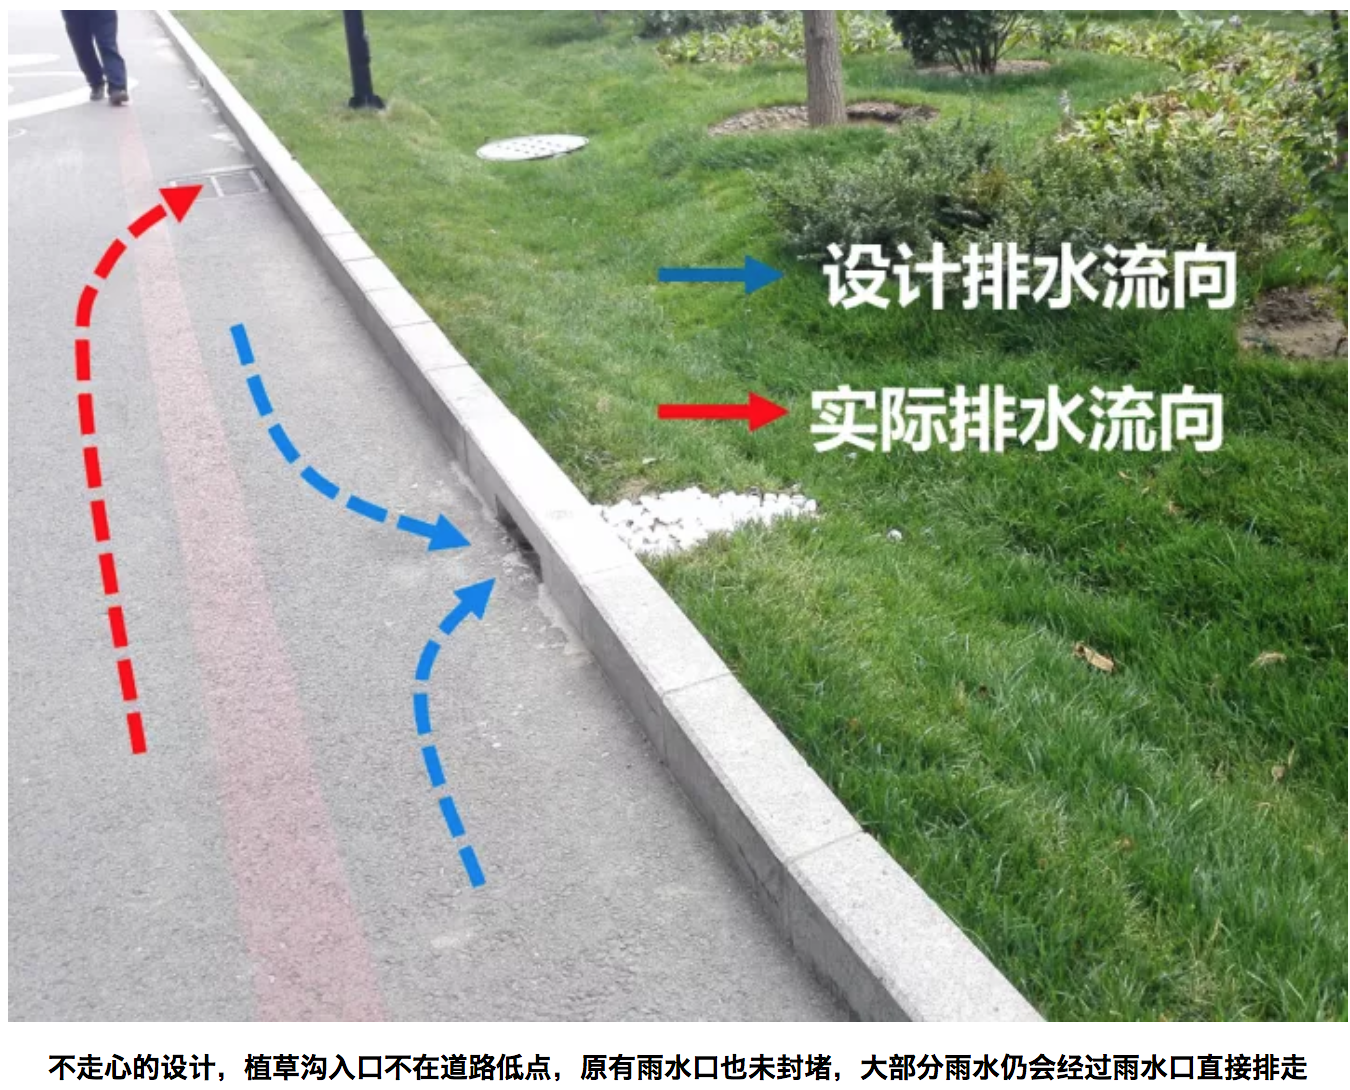
\includegraphics[width=18.75in]{images/ch7}

同时也提醒大家,海绵城市建设不只是``搞种植、搞绿化''。``花花草草''固然重要,但我们也不能天天搞``拈花惹草''的老一套。海绵城市的实质应该是绿色设施(雨水花园,植草沟,下凹式绿地等)与灰色设施(管网,泵站,调蓄池等)相结合,让它们在不同时间与空间上起到相应的功能与作用。

\subsection{结语}

海绵城市的概念一经提出,就在全国迅速地铺展开来。国内新事物的出现,不像国外``自下而上''的推进模式,而是``自上而下''的运动式推动。然而,没有前期多年的研究数据作为支撑,直接开展工程实践难免会面临各种各样的困境。
目前,``海绵城市''的提法基本已家喻户晓,无人不谈``海绵'';然而能真正潜下心来认真对海绵城市进行系统的研究与梳理的人却少之又少。一个新的领域,往往需要十年甚至更长的时间来形成系统性的理论与技术体系,之后才有可能更高效、更全面指导工程实践。希望各位海绵同仁,我们一起潜心努力,为这个领域尽自己的绵薄之力。

作者:王宇 校稿:广播站王站长 编辑:栟 手绘美图:丫头晚安

\bibliography{book.bib}



\end{document}
